% !TEX encoding = UTF-8 Unicode
\documentclass[presentation,aspectratio=169]{beamer}
\newcommand{\trans}[1]{{#1}^{\ensuremath{\mathsf{T}}}}           % transpose
\newcommand{\ci}{\ensuremath{\mathcal{I}}}
\newcommand{\abs}[1]{\left| #1\right|}                    % 
\usepackage{hyperref}
%\usepackage{movie15}
\usepackage{epstopdf}
\usepackage{colortbl}
\usepackage{amsmath}
\usepackage{amssymb}
\usepackage{pifont}
\newcommand{\cmark}{\ding{51}}%
\newcommand{\xmark}{\ding{55}}%

\usepackage{wrapfig}\usepackage{url}

\usepackage[]{graphicx}
%\input{abbrev}

\usepackage[squaren]{SIunits}
\usepackage{pgffor}
\usepackage{times}
\usepackage{pgfpages}
\usepackage[version=3]{mhchem}
\renewcommand{\angstrom}{\mbox{\normalfont\AA}}
\newcommand{\sprime}{s^\prime}
\usepackage{media9} 
\usepackage{animate}
\def\tsim{\sim}
\def\ggamma{\gamma}
\newcommand{\dd}{\mathrm{d}}
\newcommand{\shat}{\hat{s}}
\newcommand{\that}{\hat{t}}
\newcommand{\bx}{\mathbf{x}}
\newcommand{\br}{\mathbf{r}}
\newcommand{\bs}{\mathbf{s}}


\DeclareGraphicsExtensions{.jpg,.pdf,.tif,.png,.tiff,.eps}

\DeclareGraphicsRule{.tif}{png}{.png}{%
     `convert #1 `basename #1 .tif`.png%
}

\graphicspath{{./talkfigures/}}
\definecolor{uclablue}{RGB}{83,104,149}
\definecolor{osu}{RGB}{153,153,153}

\def\newblock{\hskip .11em plus .33em minus .07em}

\mode<presentation>
{
  \usetheme{Boadilla}
  %\pgfpagesuselayout{4 on 1}[letterpaper,landscape,border shrink=2.5mm]
  \usecolortheme[named=uclablue]{structure}
\useinnertheme{rounded}
  % or ...

  \setbeamercovered{transparent}
  % or whatever (possibly just delete it)
}


\usepackage[english]{babel}
% or whatever

\usepackage[utf8]{inputenc}
% or whatever

\usepackage{times}
\usepackage[T1]{fontenc}
% Or whatever. Note that the encoding and the font should match. If T1
% does not look nice, try deleting the line with the fontenc.

\newcommand{\bsigma}{\boldsymbol\sigma}

\title[APS TFM talk] % (optional, use only with long paper titles)
{Reconstruction of localized force distributions in cells and tissues from substrate displacements using physically-consistent regularization}


\author[Joshua C. Chang] {Joshua C. Chang (NIH), Yanli Liu (UCLA), Tom Chou (UCLA)}


\institute[NIH] % (optional, but mostly needed)
{
%National Institutes of Health
}
% - Use the \inst command only if there are several affiliations.
% - Keep it simple, no one is interested in your street address.

\date[March 16, 2017] % (optional, should be abbreviation of conference name)
{
APS March Meeting 2017 \\
Session S5: Machine Learning for Modeling and Control of Biological Systems I

}



%%%%%%%%%%%%%%%%%%%%%%%%%%%%%%%%%%%%%%%%%%%%%%%%%%%%%%%%%%%%%%%%%%
%%%%%%%%%%%%%%%%%%%%%%%%%%%%%%%%%%%%%%%%%%%%%%%%%%%%%%%%%%%%%%%%%%
\begin{document}

\section{Traction force microscopy}

\begin{frame}
  \titlepage
\end{frame}

%\begin{frame}{Traction force microscopy experiments}
%%\includegraphics[width=0.9\textwidth]{figures/fi}
%\end{frame}

\begin{frame}{Traction force microscopy}
\begin{columns}
\begin{column}{0.45\textwidth}
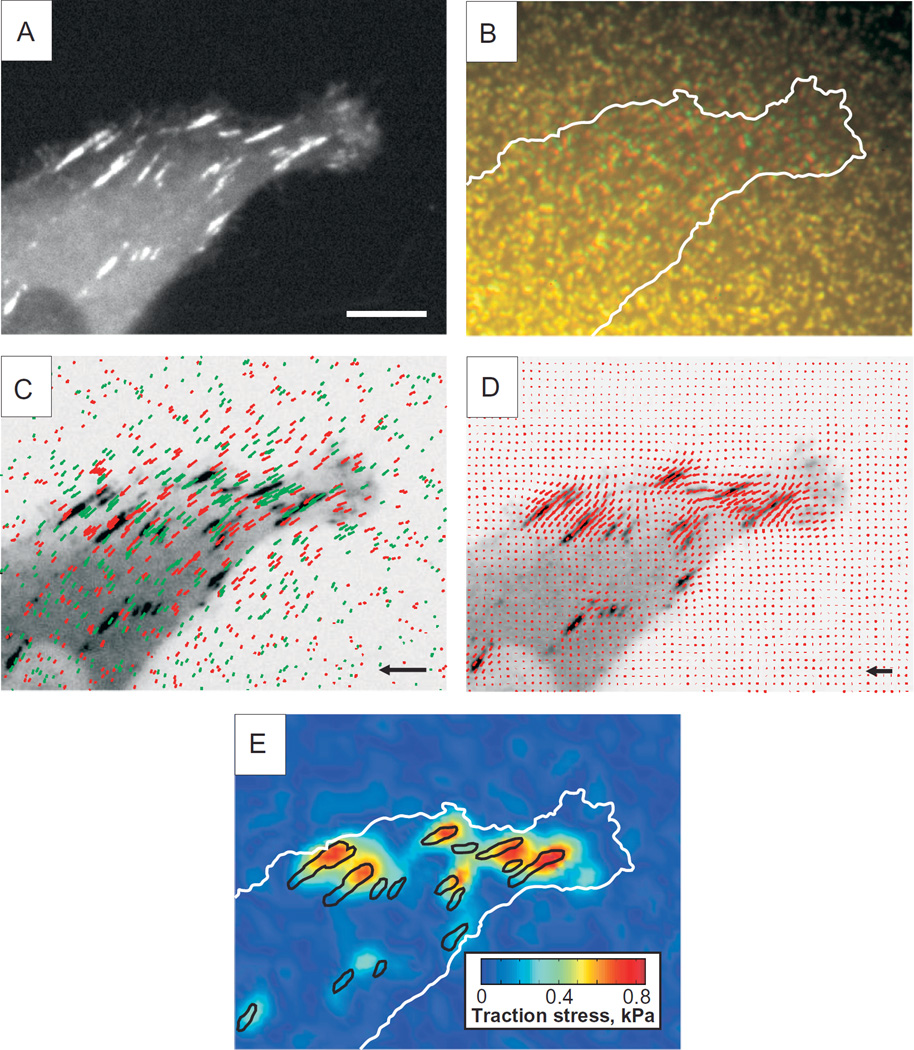
\includegraphics[width=0.9\textwidth]{figures/nihms748056f4.jpg}

\emph{Plotnikov et. al. Methods Cell Biol. 2014}
\end{column}
\begin{column}{0.55\textwidth}

Imaging focal cell adhesions by tracking the displacement of fluorescent markers placed within a medium

\bigskip

\begin{description}
\item[A] Confocal image of human breast adenocarcinoma cell
\item[B] Position of fluorescent beads
\item[C] Displacement field for beads
\item[D] Stress field
\item[E] Stress magnitude
\end{description}

\bigskip

\textbf{Goal:} Determine tangential traction stress at the surface of medium

\end{column}
\end{columns}
\end{frame}

\begin{frame}{Linear elasticity theory for displacements $\mathbf{u}$}
\begin{columns}
\begin{column}{0.65\textwidth}
\centering
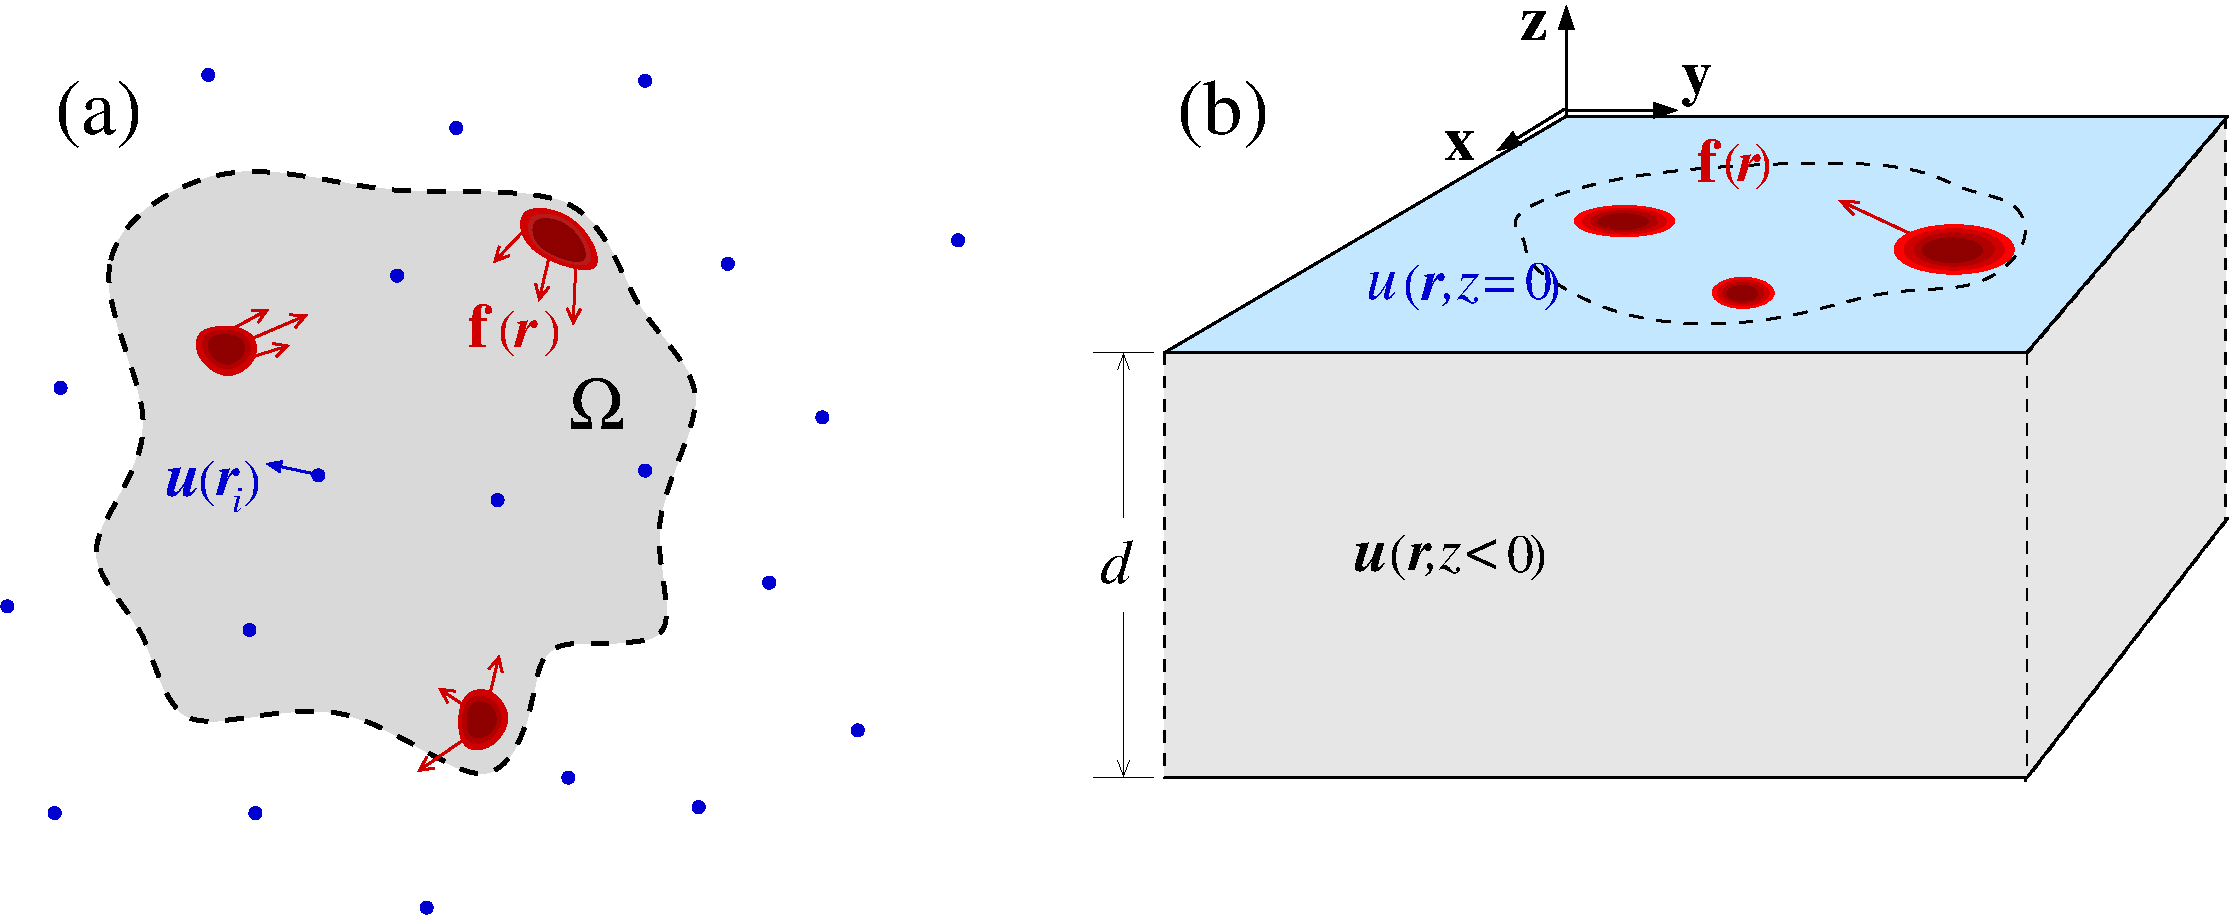
\includegraphics[width=\textwidth]{figures/Fig1}
\end{column}
\begin{column}{0.35\textwidth}
\begin{itemize}
\item $\bsigma$ is tangential surface stress tensor, proportional to the $\mathbf{F}_\perp$
\item $\mathbf{u}$ found ``exactly'' in closed-form for any fixed piecewise-polynomial approximation of $\bsigma$
\end{itemize}
\end{column}
\end{columns}

\scriptsize

\begin{block}{In-plane surface displacements, as $d\to\infty,$ where $G \propto (Er)^{-1}$}
\vspace{-10pt}
\begin{align*}\tiny
u_{x}(x,y) &= \int_\Omega \dd x'\dd y'G_{xx}( x-x',y-y')\sigma_{xz}(x',y') 
 +  \int_\Omega \dd x'\dd y'G_{xy}( x-x',y-y')\sigma_{yz}(x',y')  \\
u_y(x,y) &= \int_\Omega \dd x'\dd y'G_{yx}( x-x',y-y')\sigma_{xz}(x',y') +  \int_\Omega \dd x'\dd y'G_{yy}( x-x',y-y')\sigma_{yz}(x',y') 
\end{align*}
\end{block}

\end{frame}

\begin{frame}{Discretized forward problem}
 \small
\begin{block}{Linear algebra system}
\begin{itemize}
\item $\boldsymbol\sigma$ interpolated about points $\bs_i$ (using polynomials)
\item Solution exact up to order of interpolation of $\boldsymbol\sigma_i$
\end{itemize}
\begin{columns}
\begin{column}{0.55\textwidth}
\[
\underbrace{\left(\begin{matrix} 
u_{x}({\br_1} )\\
u_x({\br_2} ) \\
\vdots \\
u_x({\br_N} ) \\
u_{y}({\br_1} )\\
u_y({\br_2} ) \\
\vdots \\
u_y({\br_N} )
\end{matrix}\right)}_{2N\times1} =
\overbrace{\left(\begin{matrix}
\mathbb{G}_{xx} & \mathbb{G}_{xy} \\
\mathbb{G}_{yx} & \mathbb{G}_{yy}
\end{matrix}\right)}^{\mathbb{G}}
\underbrace{\left(\begin{matrix} 
\sigma_{xz}({\bs_1} )\\
\sigma_{xz}({\bs_2} ) \\
\vdots \\
\sigma_{xz}({\bs_M} ) \\
\sigma_{yz}({\bs_1} )\\
\sigma_{yz}({\bs_2} ) \\
\vdots \\
\sigma_{yz}({\bs_M} )
\end{matrix}\right)}_{2M\times1} 
\]
\end{column}
\begin{column}{0.4\textwidth}
\begin{itemize}
\item $\{\mathbf{r}_i\}_{i=1}^N$  locations at which measurements are taken
\item $\{\mathbf{s}_i\}_{i=1}^M$  locations controlling interpolation of $\boldsymbol\sigma$
\item $\mathbb{G}$ composed of grid-cell moments of the Greens function
\item  $\mathbb{G}$ depends on the interpolation order of $\boldsymbol\sigma$
\end{itemize}
\end{column}
\end{columns}
\end{block}
\end{frame}




\begin{frame}{Using the physics to help constrain the inverse problem}
\small
\begin{columns}
\begin{column}{0.4\textwidth}
\begin{block}{Reasonable physical assumptions}
\begin{enumerate}
\item No force outside the cell footprint
\item No inertia (forces and torques each sum to zero)
\end{enumerate}
\end{block}
\end{column}
\begin{column}{0.5\textwidth}
 
\begin{block}{Advantage gained}
\begin{enumerate} \scriptsize
\item Reduction in problem size
\begin{itemize} \scriptsize
\item Throw away far data points
\end{itemize}
\item Multipole expansion $\Rightarrow$  decay at rate $r^{-2}$
\begin{itemize} \scriptsize
\item Cutoff data by distance
\item Sparsify the matrix $\mathbb{G}$
\end{itemize}
\end{enumerate}
\end{block}
\end{column}
\end{columns}

\begin{exampleblock}{Still need to regularize the inverse problem}

\begin{columns}
\begin{column}{0.4\textwidth}

Criteria for a well-posed problem
\begin{itemize}
\item Solution exists
\item Solution unique
\item Solution continuous w.r.t. data
\end{itemize}
\end{column}
\begin{column}{0.55\textwidth} \Large
\[
\hat{\boldsymbol\sigma} = \arg\min_{\boldsymbol\sigma}\left[ \underbrace{||\mathbf{u} - \mathbb{G}\mathbf{\bsigma}  ||_2^2}_{\Phi_{\textrm{data}}} + \lambda\Phi_{\textrm{reg}}[\boldsymbol\sigma] \right]
\]
\end{column}
\end{columns}

\end{exampleblock}

\end{frame}

 
\begin{frame}{Respecting the physics in regularizing the inverse problem}
\small
\begin{itemize}
\item \textbf{Principle:} Coordinate system should not bias results
\item \textbf{Solution:}  Regularize using functionals of the tensor invariants
\end{itemize}
\begin{columns}
\begin{column}{0.35\textwidth}
\begin{exampleblock}{Tensor invariants}
\[
\textrm{Tr}(\boldsymbol\sigma) = \sigma_{xz} + \sigma_{yz}
\]
\[
\textrm{Det}(\boldsymbol\sigma) = \sigma_{xz}\sigma_{yz}
\]
\end{exampleblock}
\end{column}
\begin{column}{0.6\textwidth}
\begin{exampleblock}{Invariant regularization functionals $\Phi_{\textrm{reg}}$}
\[
\Phi_{L^1(Tr)} = \int_\Omega \vert \sigma_{xz}(x,y) + \sigma_{yz}(x,y)  \vert \dd x\dd y
\]
\[
\Phi_{TV(Tr)} =  \int_\Omega | \nabla(\sigma_{xz}(x,y) + \sigma_{yz}(x,y) ) | \dd x\dd y.
\]

\end{exampleblock}
\end{column}
\end{columns}
\begin{block}{Non-invariant functionals $\Phi_{\textrm{reg}}$} \small
\[
\Phi_{L1} = \int_\Omega\left( \left| \sigma_{xz}(x,y) \right|+\left|\sigma_{yz}(x,y) \right|\right)\dd\bx,
\]
\[
 \Phi_{TV_1} = \int_\Omega \left( \vert\nabla\sigma_{xz}(x,y) \vert + \vert\nabla\sigma_{yz}(x,y) \vert\right)\dd\bx
\qquad
\Phi_{TV_2} = \int_\Omega  \left( \vert\partial_x\sigma_{xz}\vert + \vert\partial_y\sigma_{xz}\vert + \vert\partial_x\sigma_{yz}\vert+ \vert\partial_y\sigma_{yz}\vert\right)\dd\bx
\]

\end{block}

\end{frame}

 \begin{frame}{High-resolution data}
 \begin{columns}
 \begin{column}{0.35\textwidth}
 \begin{itemize}
  \item Mesenchymal stem cell
 \item Polyacrylamide hydrogels
 \item  Fluorescent beads in a regular grid
 \item High-resolution measurement of displacement field
 \item Cell boundary estimated from raw bright-field image (superimposed)
 \end{itemize}
 \end{column}
 \begin{column}{0.7\textwidth}
 \centering
 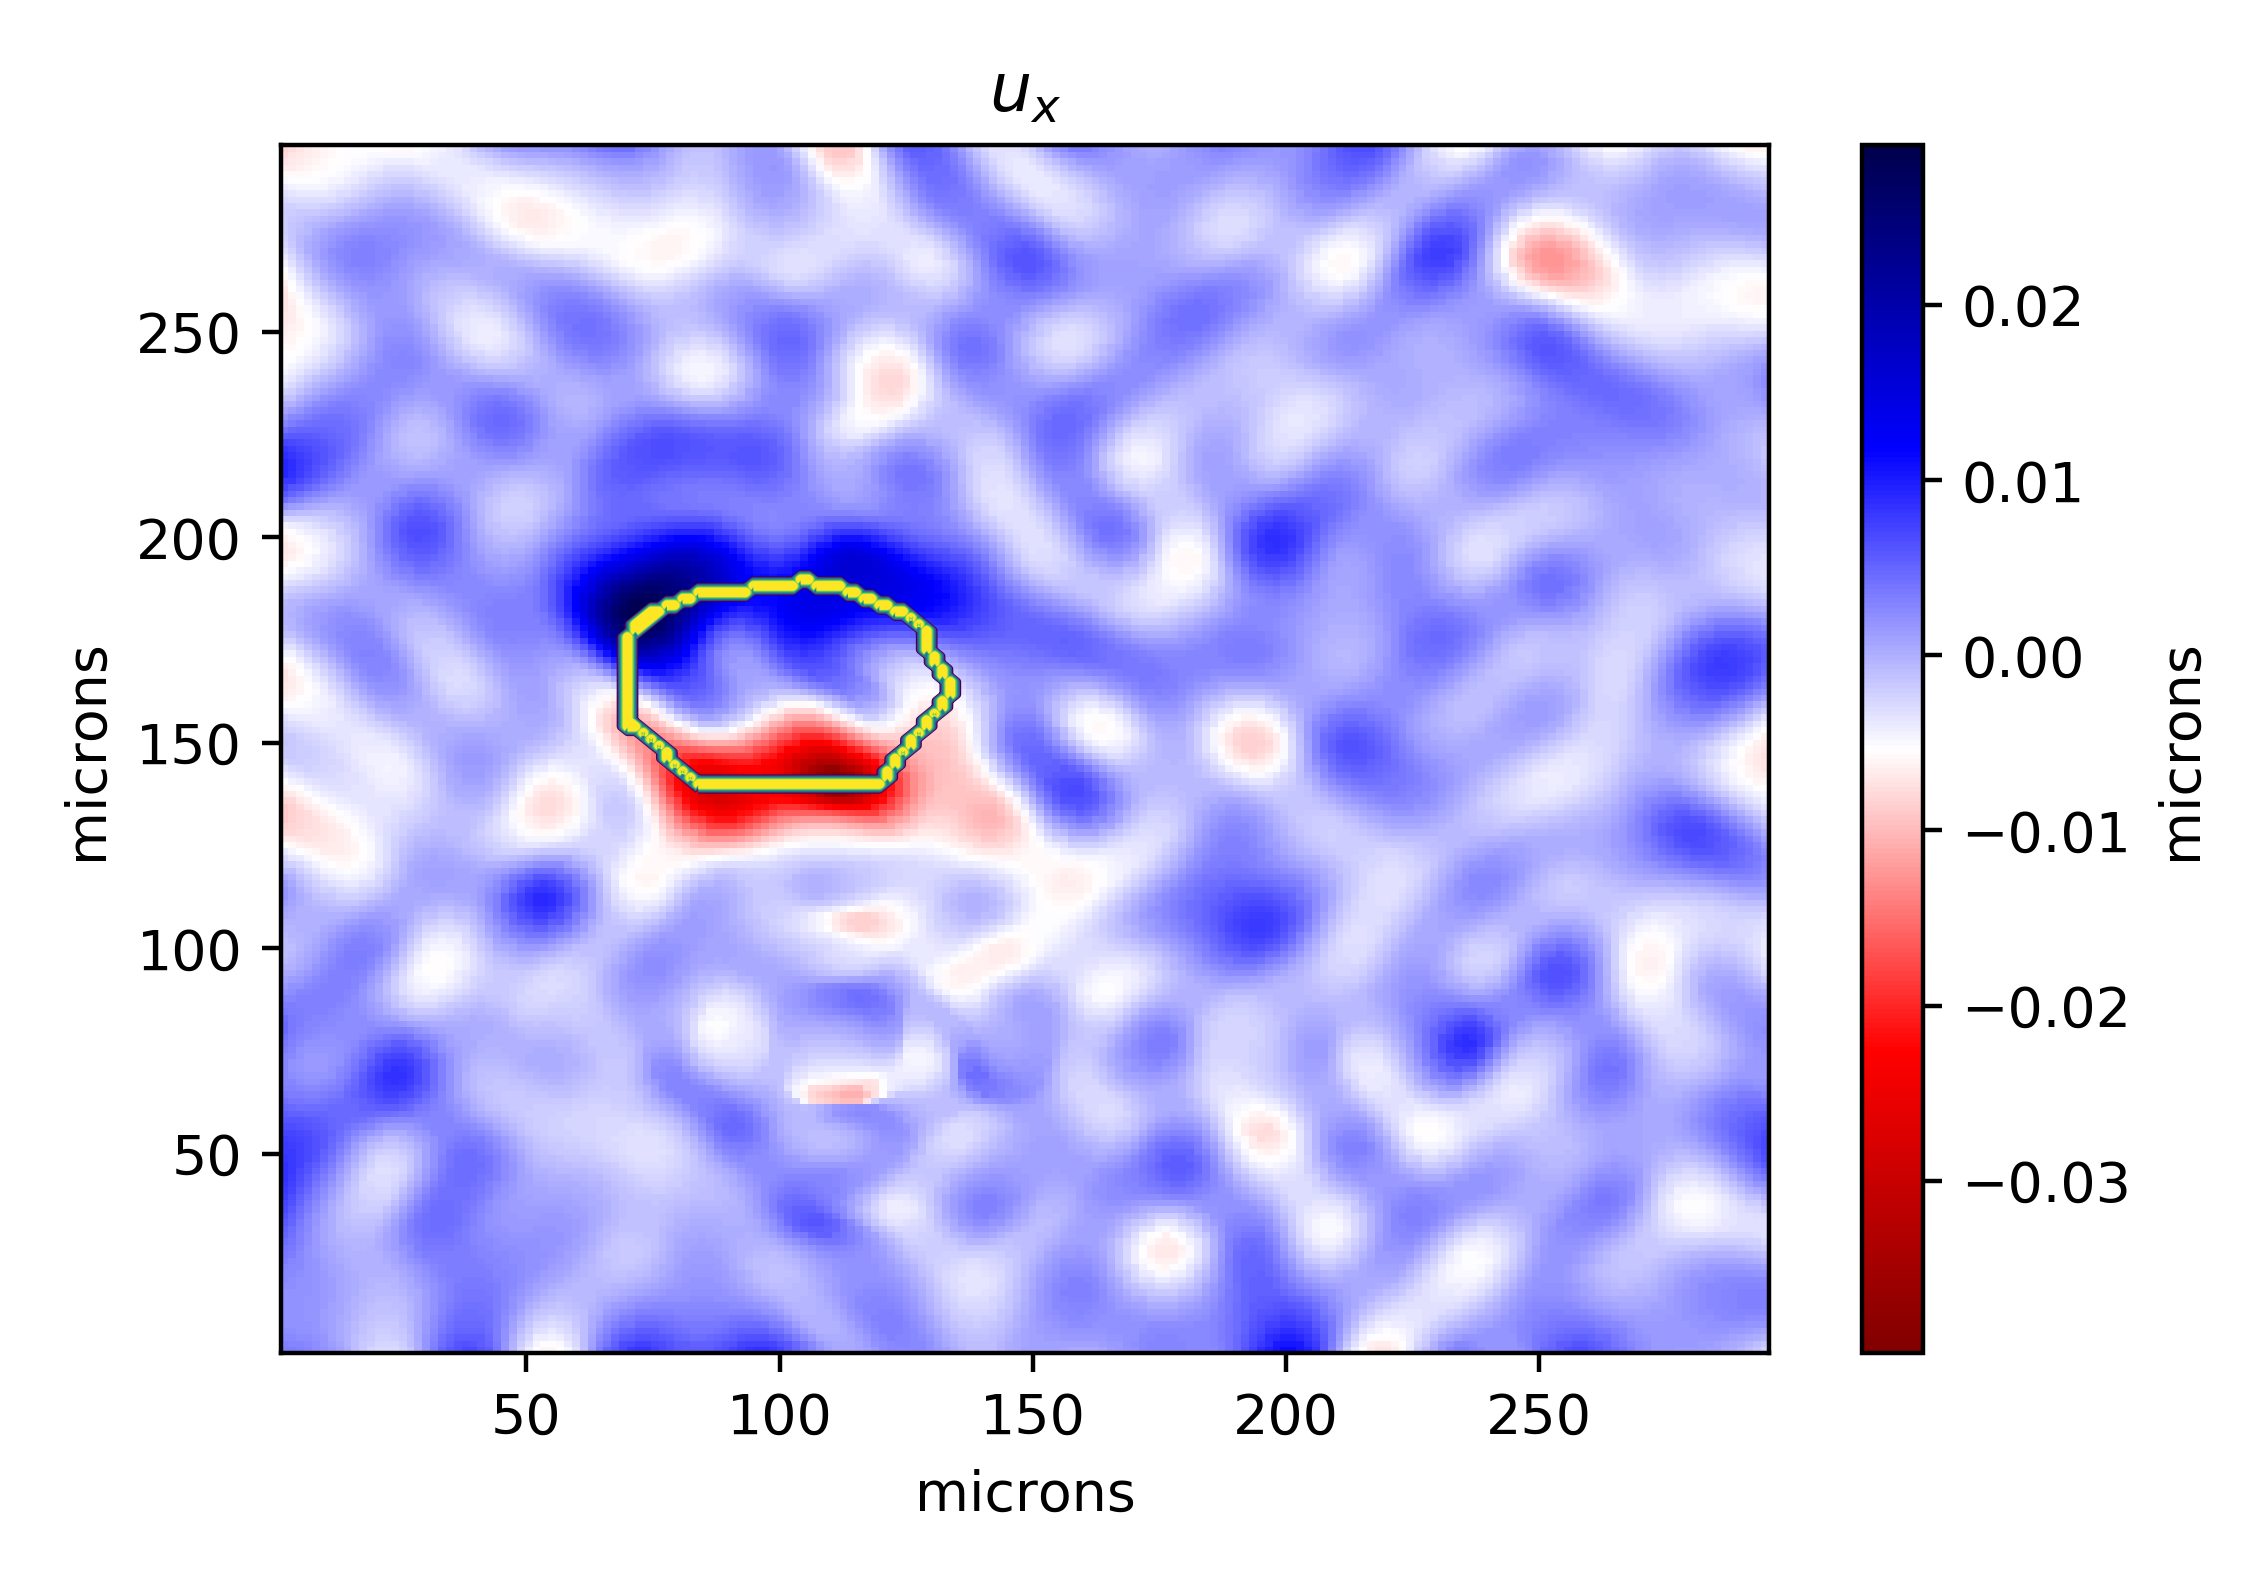
\includegraphics[width=0.9\textwidth]{figures/fig0a}
  
 \emph{Courtesy of Gabriel Popescu, UIUC}
  \end{column}
  \end{columns}
 \end{frame}
 
\begin{frame}{Rotational invariance matters}
\centering
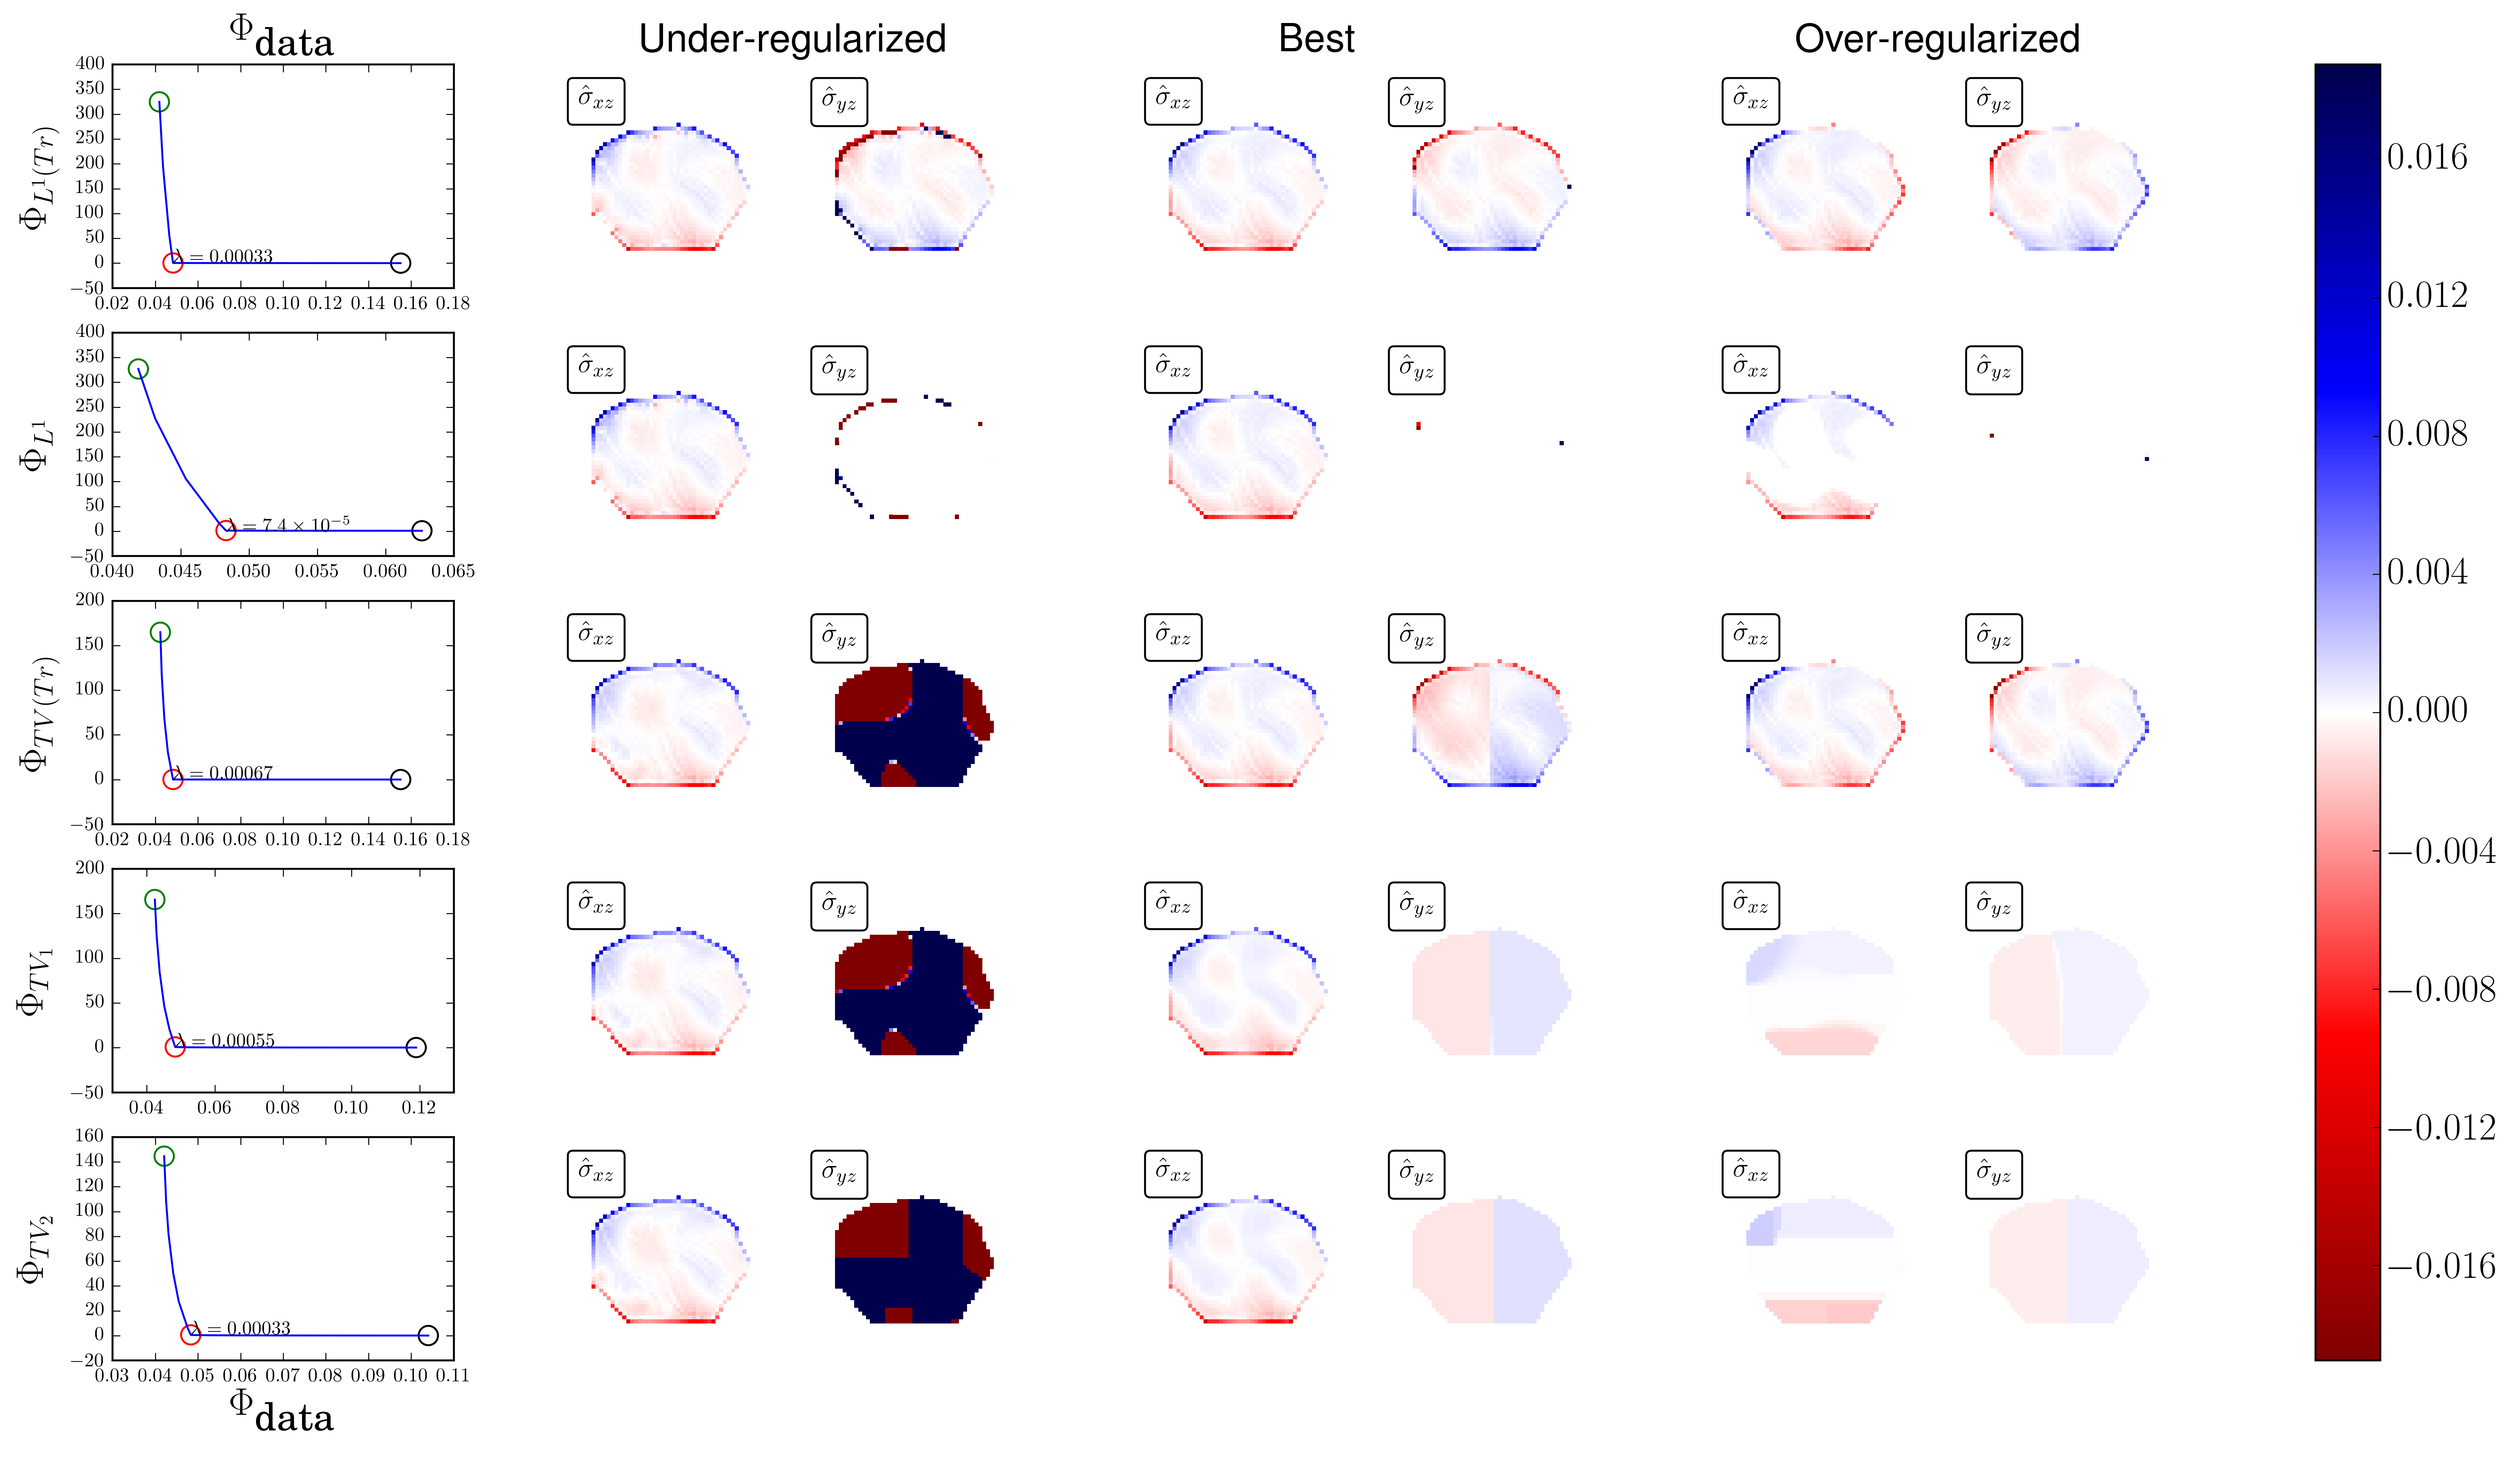
\includegraphics[width=0.88\textwidth]{figures/fig2}\ \rotatebox{90}{\scriptsize \qquad\qquad\qquad\qquad \emph{Units:} $E\textrm(Young's\ modulus)$}
\end{frame}

\begin{frame}{Force constraints matter}
\centering
\begin{columns}
\begin{column}{0.6\textwidth}
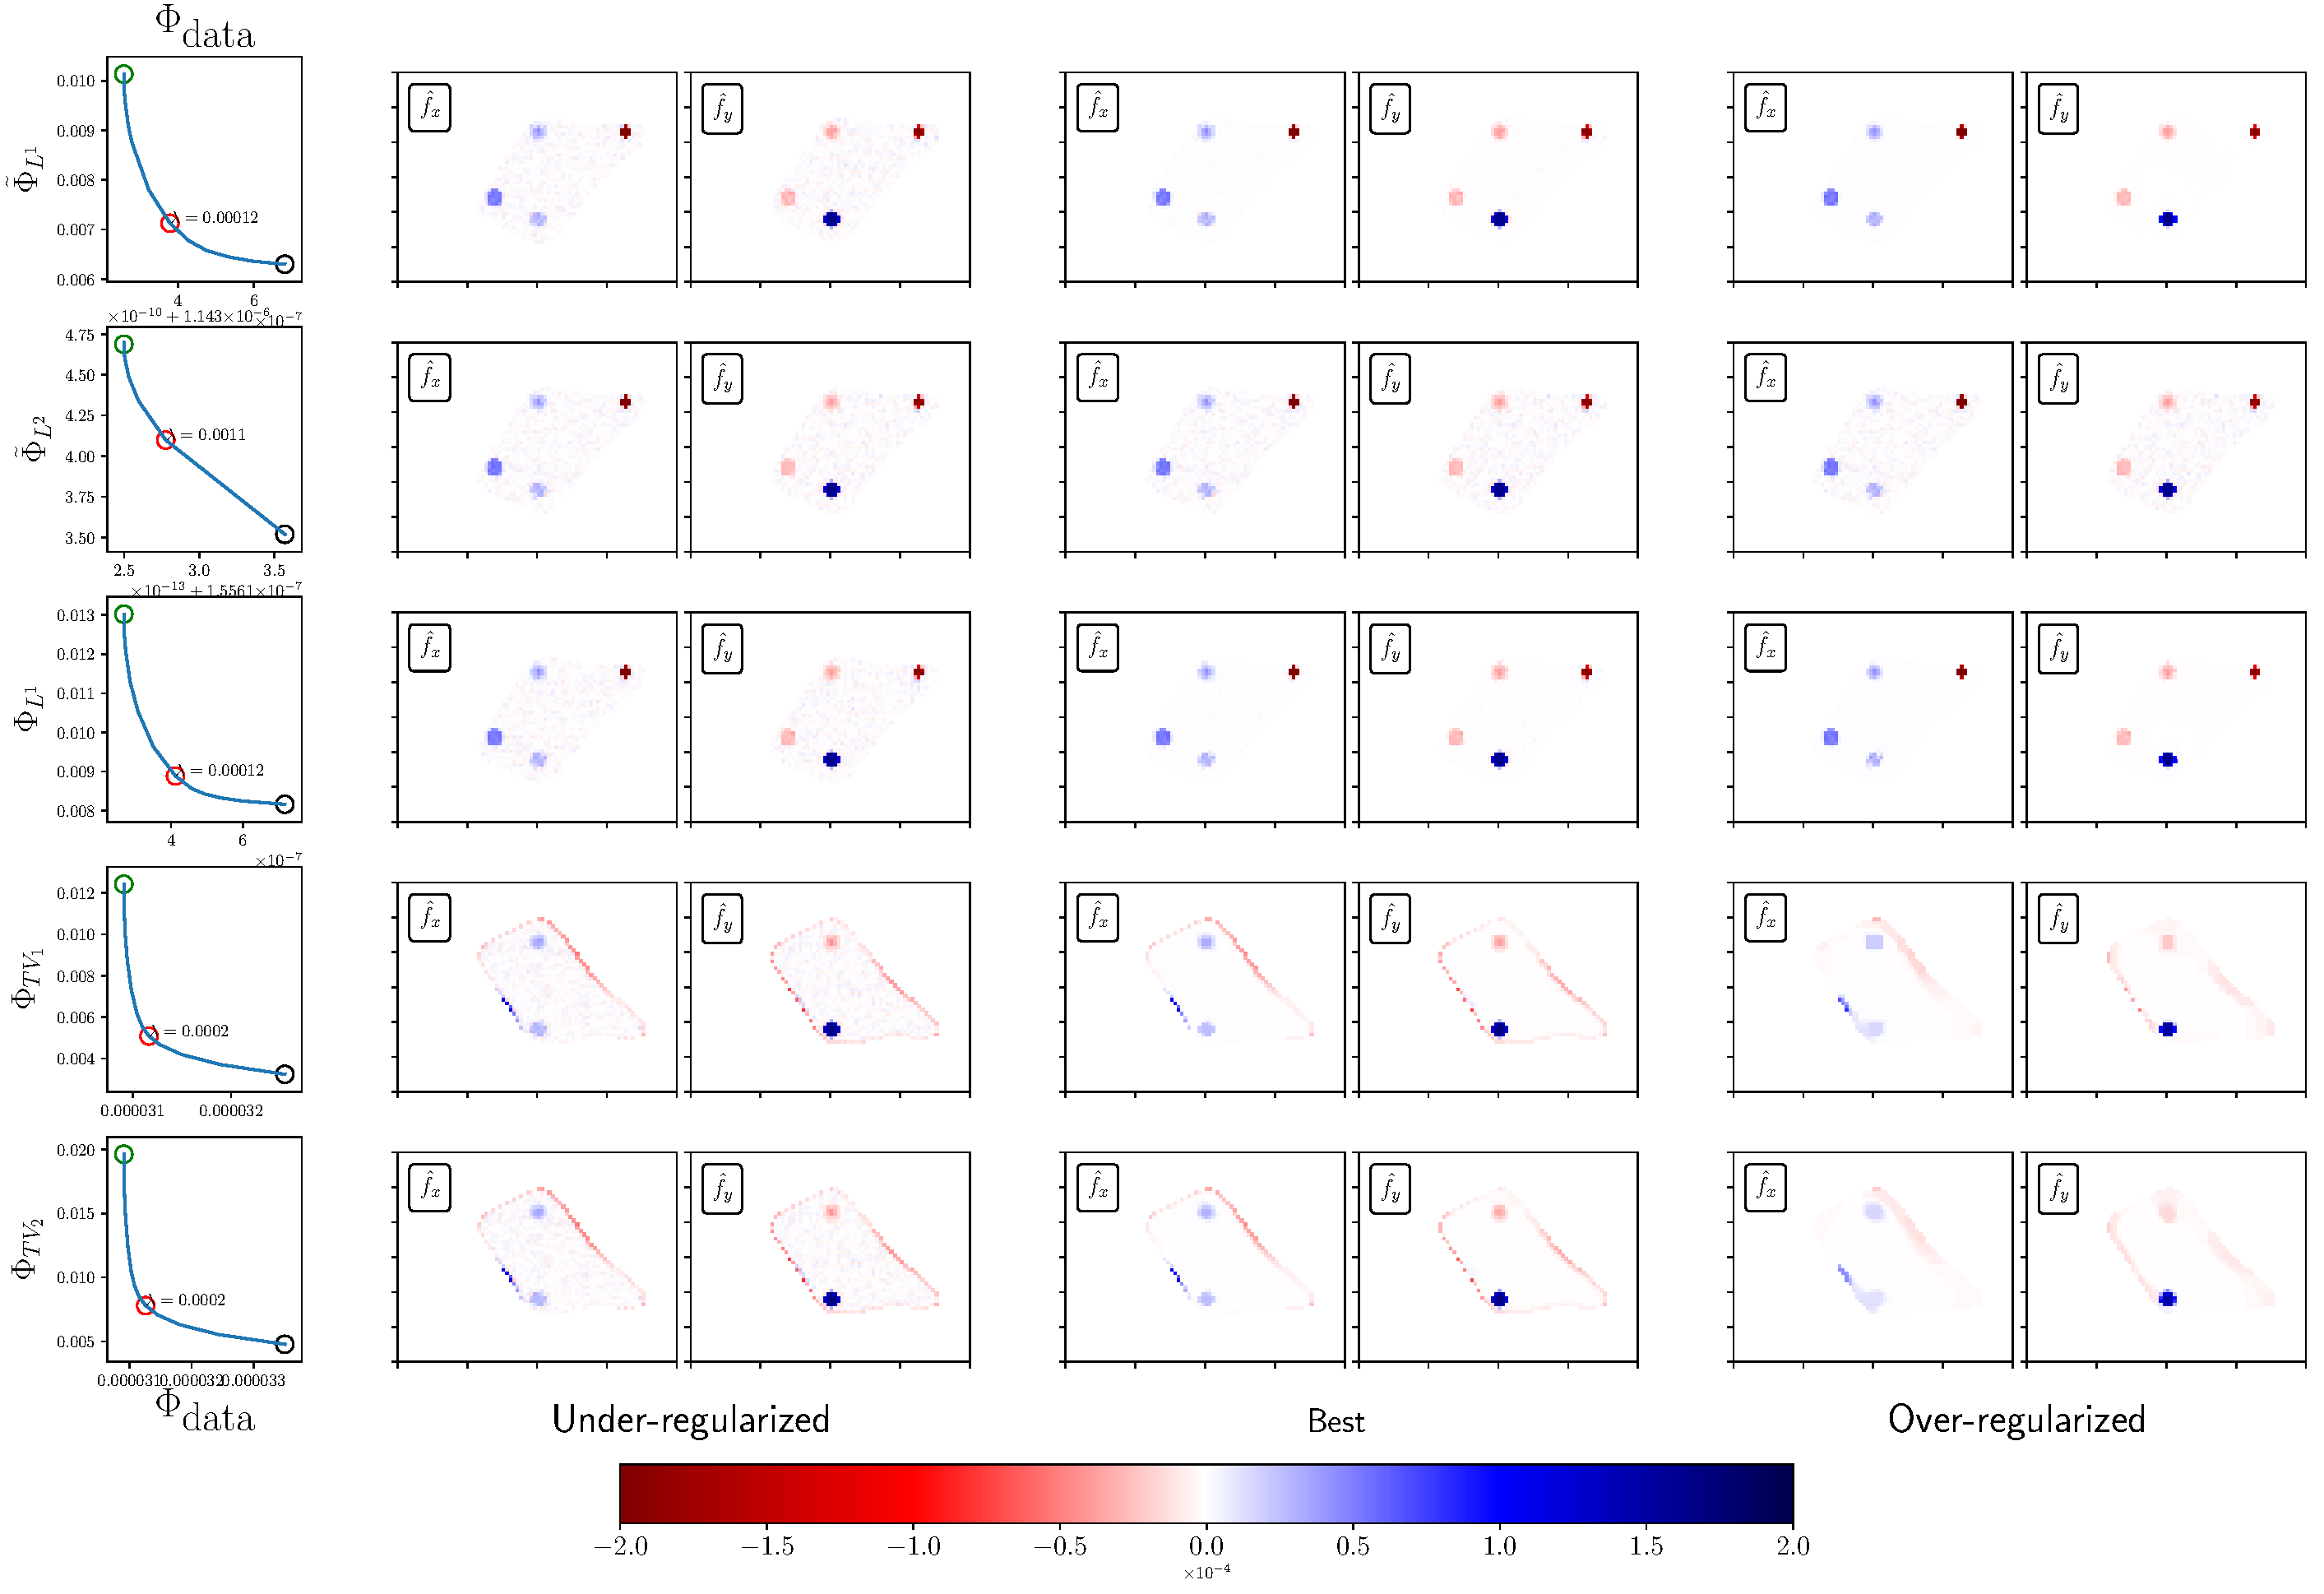
\includegraphics[width=\textwidth]{figures/fig3}
\end{column}
\begin{column}{0.4\textwidth}
\begin{itemize}
\item Reconstructions performed using $L_1(Tr)$
\item Difference compared to fully-constrained reconstruction
\item Neither force nor torque cancel unless enforced explicitly
\end{itemize}
\end{column}
\end{columns}
\end{frame}

\begin{frame}{The footprint constraint matters}
\centering
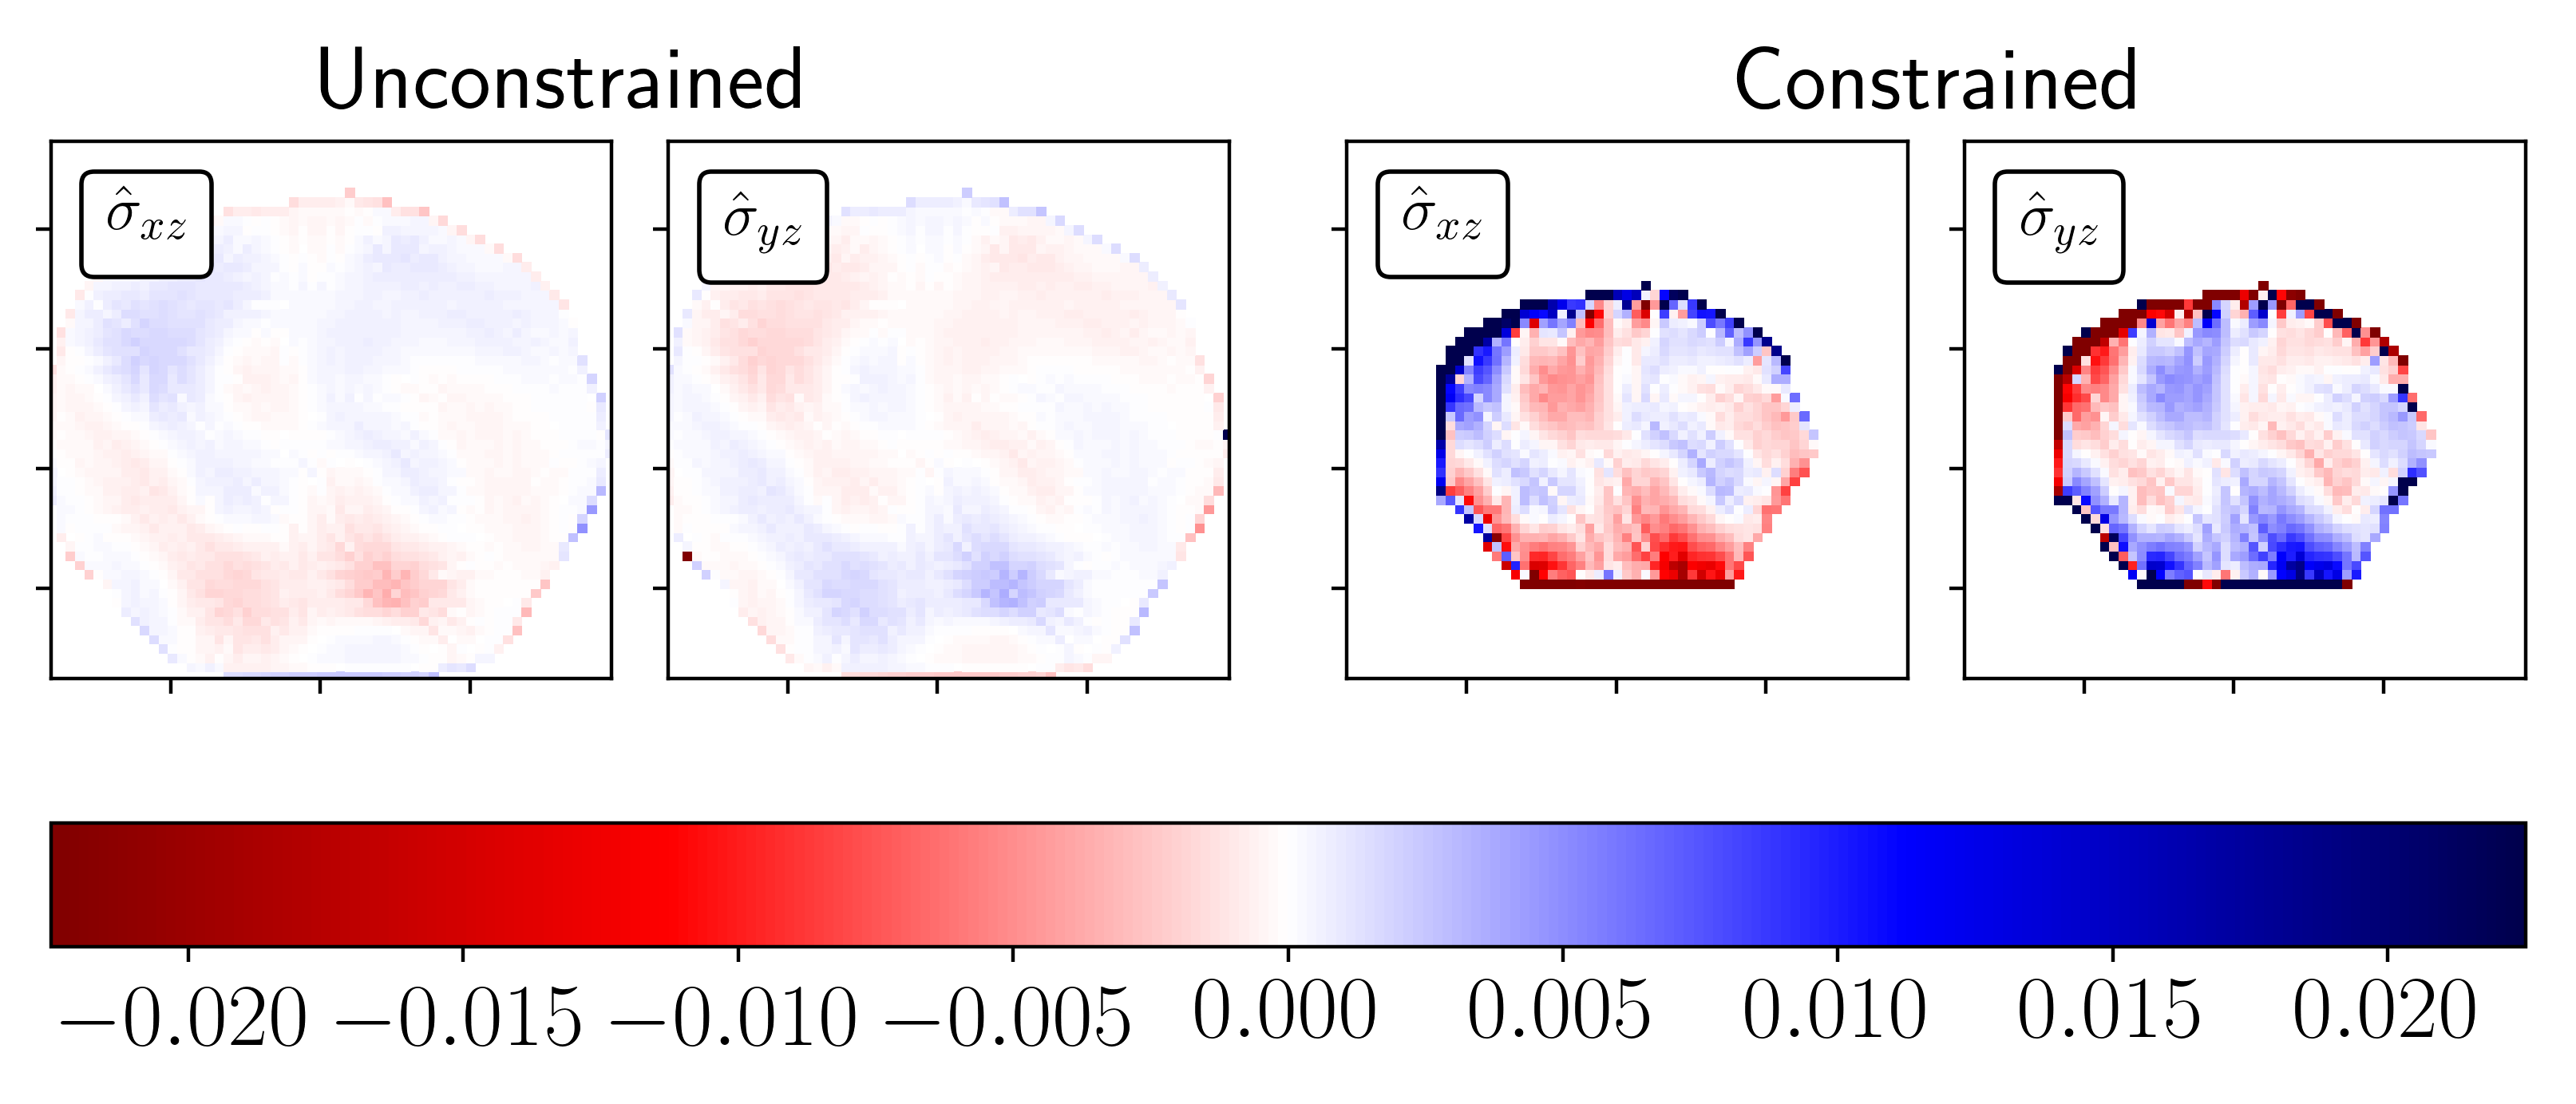
\includegraphics[width=0.9\textwidth]{figures/fig4}
\begin{itemize}
\item Force concentrated near edges of the cell
\item Location of edges is important
\end{itemize}
\end{frame}

\begin{frame}{Summary and Future directions}
\begin{itemize}
\item The regularization should be consistent with the known physics (as in a Bayesian prior)
\item The numerical solution of the forward problem should be consistent with the regularization
\item Localization of the cell footprint is important in determining traction
\begin{itemize}
\item Extension: Joint force reconstruction and cell boundary determination
\item Extension: Uncertainty quantification through Bayes
\end{itemize}
\end{itemize}

\centering



\smallskip
\emph{From the authors:} {Joshua C. Chang (NIH), Yanli Liu (UCLA), Tom Chou (UCLA)}, 

\smallskip
Thank you!

\smallskip

\emph{Funding:} NIH Intramural Research Program, ARO, NSF

\end{frame}



\end{document}


